\chapter{MATLAB程序设计语言与初等数学运算}
\begin{introduction}
\item 变量与数据类型
\item 数据~/~图形输出
\item 逻辑运算
\item 函数
\item 控制语句
\end{introduction}

\begin{note}
本章内容较繁杂,仅列举考试主体,细节请各位自行翻阅课本及课件!
\end{note}

\section{变量与数据}
\subsection{变量与数据}
\begin{itemize}
  \item 命名规则
  \item 常用变量
\end{itemize}
\subsection{数据类型}
\begin{itemize}
  \item 数值(向量、矩阵,用~[]~标识,注意区分~,~~/~~\verb*+ +与~;~)
  \item 字符(用'\mlplaceholder{string}'标识)
  \item 单元数组,cell array(注意'\{\}'的使用方法)
  \item 结构体,structure(用'.'标识)
  \item 函数句柄
\end{itemize}
\subsection{生成向量}
\begin{lstlisting}[frame=single,numbers=left]
a=1:10 %默认以1为间距
a=1:2:10 %以2为间距
% 线性等分
y=linspace(`\mlplaceholder{start}`,`\mlplaceholder{end}`(,`\mlplaceholder{n}`))
% 对数等分
y=logspace(`\mlplaceholder{start}`,`\mlplaceholder{end}`(,`\mlplaceholder{n}`))
\end{lstlisting}
\newpage
\section{数据输出}
\subsection{disp函数}
\begin{lstlisting}[frame=single,numbers=left]
%显示`\mlplaceholder{X}`到屏幕,并自动换行
disp(`\mlplaceholder{X}`)
% 输出矩阵
a=[1 2;3 4];
disp(a)
% 输出字符
disp('A') %将输出字母A
disp(['1+1=',num2str(2)]) %使用 [] 连接字符
\end{lstlisting}

\subsection{fprintf函数}

\begin{definition}{常用转义字符}{}
\%n~换行~~~\%t制表符~~~\%f固定位数小数~~~\%s~字符或字符串~~~\%e~指数形式
\end{definition}
举例如下:
\begin{lstlisting}
% Work2_4 计算压降
L=3000;d=45;V=1600;
deltP=0.03*L*(V/1000)^1.84/d^1.24;
disp('L=3000m d=45mm V=1600m/min')
disp('压降计算值为:')
fprintf('\tdeltP=%.2e\n',deltP)
\end{lstlisting}
\begin{figure}[htbp]
	\centering
	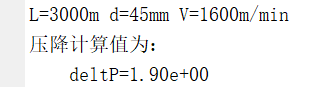
\includegraphics[width=0.6\textwidth]{fprintf.png}
	\caption{运行结果}
\end{figure}
\newpage
\section{图形输出}
\subsection{基本概念}
\begin{lstlisting}[frame=single,numbers=left]
% 可将多条曲线绘制于同一图形窗口
% '`\mlplaceholder{S}`'对线型、颜色、数据点形貌等设置
% 线型 -实线  :虚线  -.点划线 --双画线
% 颜色 b蓝色 g绿色 r红色 k黑色
% 点貌 .黑心实点 o空心圆圈 p五角星符
plot(`\mlplaceholder{X1}`,`\mlplaceholder{Y1}`,'`\mlplaceholder{S1}`',`\mlplaceholder{X2}`,`\mlplaceholder{Y2}`,'`\mlplaceholder{S2}`',…)
\end{lstlisting}
示例如下:
\begin{figure}[htbp]
	\centering
	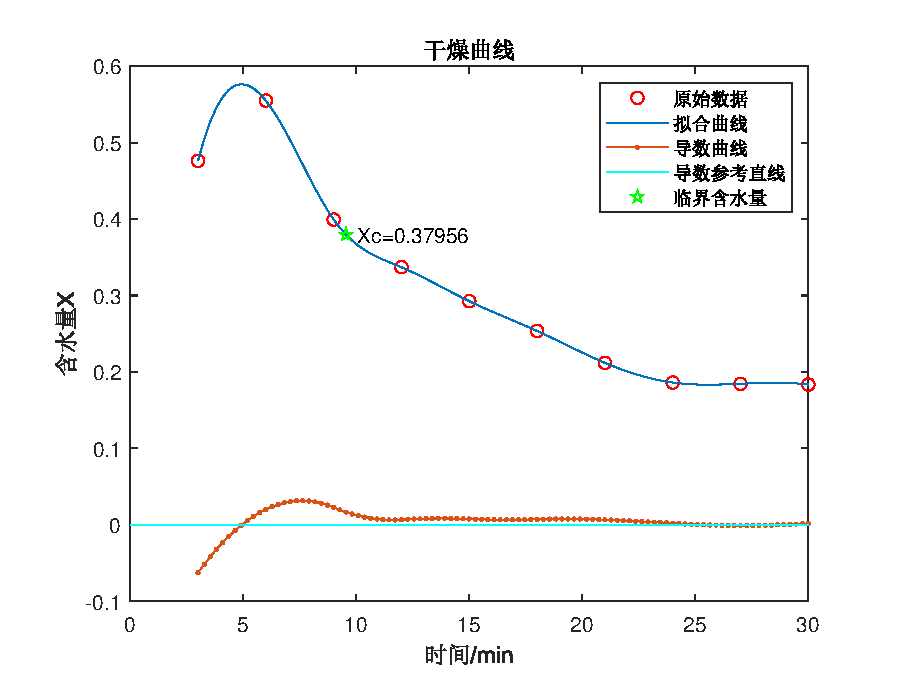
\includegraphics[width=1\textwidth]{plot.eps}
	\caption{运行示例}
\end{figure}
\newpage
\begin{lstlisting}
% 数据来自上机材料5 3.1
function exam5_3_1
t=3:3:30;
G1=[10.2 13.9 12.16 13.49 13.74 12.01 11.55 11.02 12 12.12];
G2=[6.91 8.94 8.69 10.09 10.63 9.58 9.53 9.29 10.13 10.24];
A=1.83;
X=(G1-G2)./G2;
tt=linspace(3,30);
% 插值
pp=spline(t,X);
ppv=fnval(pp,tt);
plot(t,X,'ro') %绘制原始数据,红色圆圈
hold on %保持图形窗口,继续绘制曲线
plot(tt,ppv) %绘制拟合曲线,观察插值结果
% 微分
figure %打开新图形窗
dp=fnder(pp);
dpv=-fnval(dp,tt)./A;% 干燥速率
plot(t,X,'ro',tt,ppv,tt,dpv,'.-') %同时绘制两条曲线
axisX=refline(0,0) %绘制斜率0,截距0的参考直线
axisX.Color='c'
% 计算临界含水量并标注
Um=max(dpv);
loc=find(dpv>Um/2,1,'last'); %临界含水量在向量中索引
tc=tt(loc);% 临界时间
hold on
plot(tc,ppv(loc),'gp') %临界含水量
% 图名
title('干燥曲线')
% 添加图例
legend('原始数据','拟合曲线','导数曲线','导数参考直线','临界含水量')
% 设置坐标轴
xlabel('时间/min')
ylabel('含水量X')
% 文字标注
text(tc+0.5,ppv(loc),strcat('Xc=',num2str(ppv(loc))))
\end{lstlisting}
\section{函数}
\subsection{基本用法与子函数}
\begin{lstlisting}[frame=single,numbers=left]
% 注意:[]与()的使用
function [`\mlplaceholder{y1}`,`\mlplaceholder{y2}`,..]=FunName(`\mlplaceholder{x1}`,`\mlplaceholder{x2}`,..)
%主函数下,没有输入,只有输出的子函数,如果不位于末尾,需要写end
%仅能在主函数内部调用,无法在外部调用
function y=SubFunName
\end{lstlisting}
\subsection{匿名函数}
函数$f(x,y)=x^2+y^2=-1$可表示如下:
\begin{lstlisting}[frame=single,numbers=left]
f=@(x,y) x^2+y^2-1;
f(1,2) %输出为4
\end{lstlisting}
\section{关系与逻辑运算}
\subsection{主要运算符与函数}
\textbf{关系操作符}:==、~=、>

\textbf{关系运算函数}:find()~非零元素下标
\begin{lstlisting}
a=[1 2 3];
find(a>=2) %输出为[2 3]
\end{lstlisting}

\textbf{逻辑运算}:\& (与)~~~|~(或)~~~\~{}~(非)~~~xor~(异或)
\begin{lstlisting}
a=[0 1 1];b=[0 0 1];
find(a&b) %输出为 3
\end{lstlisting}
\subsection{优先级}
\begin{figure}[htbp]
	\centering
	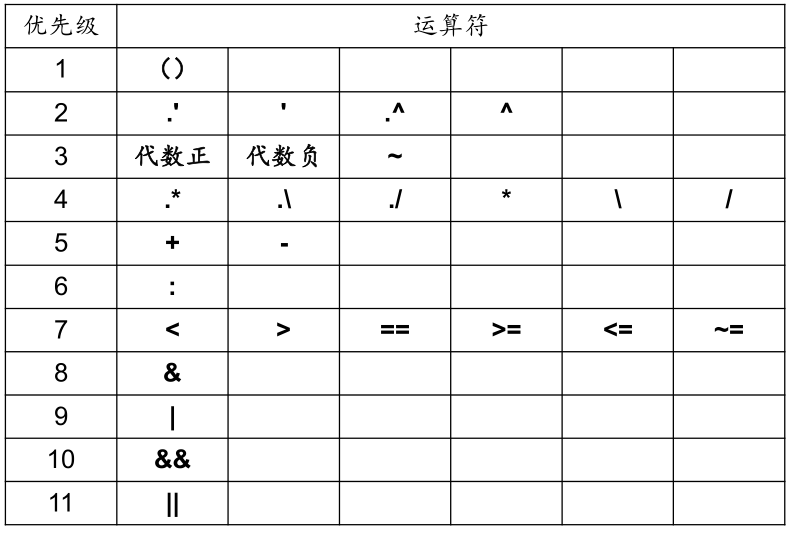
\includegraphics[width=0.6\textwidth]{priority.png}
	\caption{运算优先级}
\end{figure}
\newpage
\section{MATLAB程序控制}
\subsection{if选择语句}
\begin{lstlisting}[frame=single,numbers=left]
if `\mlplaceholder{condition1}`
    `\mlplaceholder{statements1}`
elseif `\mlplaceholder{condition2}`
    `\mlplaceholder{statements2}`
else
    `\mlplaceholder{statements3}`%譬如error(`\mlplaceholder{报错内容}`)
end
\end{lstlisting}
\subsection{for循环语句}
\begin{lstlisting}[frame=single,numbers=left]
for `\mlplaceholder{循环变量}`=`\mlplaceholder{初值}`:`\mlplaceholder{步长}`:`\mlplaceholder{终值}`
    `\mlplaceholder{循环语句}`
end
\end{lstlisting}
\subsection{whlie循环语句}
\begin{lstlisting}[frame=single,numbers=left]
while `\mlplaceholder{条件表达式}`
    `\mlplaceholder{循环语句}`
end
\end{lstlisting}
\begin{note}
了解continue、break、return函数的作用。break跳出该层循环,continue进入该层循环的下一次迭代,return退出程序或函数返回。
\end{note}